\documentclass[10pt, xcolor=table]{beamer}

\usepackage[utf8]{inputenc}
\usepackage{amsmath}
\usepackage{amsfonts}
\usepackage{amssymb}
\newcommand*\themecol{\usebeamercolor[fg]{structure}}

\setbeamertemplate{navigation symbols}{}
 \setbeamertemplate{footline}[frame number]

\newcommand{\overbar}[1]{\mkern 1.5mu\overline{\mkern-1.5mu#1\mkern-1.5mu}\mkern 1.5mu}

\usepackage{tikz}
\usetikzlibrary{shapes.geometric, arrows}
\tikzstyle{prob} = [rectangle, minimum width=3cm, text width = 4.5cm, minimum height=1cm, text centered, draw=black, fill= blue!20]
\tikzstyle{stat} = [rectangle, minimum width=3cm,  text width = 4.5cm, minimum height=1cm, text centered, draw=black, fill= red!20]
\tikzstyle{arrow} = [thick,->,>=stealth]


\setlength{\parindent}{0pt}
\setlength{\parskip}{6pt}

\title{STAT 111\\
{\small Recitation 4}}

\author{Mo Huang}
\institute{Email: mohuang@wharton.upenn.edu \\
\vspace{0.25cm}
Office Hours: Wednesdays 3:00 - 4:00 pm, JMHH F96\\
\vspace{0.25cm}
Slides: \url{github.com/mohuangx/STAT111-Spring2019} }


\date{February 15, 2019}


\begin{document}

\begin{frame}
\titlepage
\end{frame}


\begin{frame}{Many Random Variables}
\begin{itemize}
\setlength{\itemsep}{15pt}
\item Let $X$ and $Y$ be two random variables. Then,
\vspace{0.25cm}
\begin{itemize}
\setlength{\itemsep}{10pt}
\item[] {\color{blue}$\text{mean}(X + Y) = \text{mean}(X) + \text{mean}(Y).$} 
\item If $X$, $Y$ are also independent,
\item[] {\color{blue}$\text{variance}(X +Y) = \text{variance}(X) + \text{variance}(Y).$}
\item For constants $a, b$, we have
\item[] {\color{blue}$\text{mean}(aX + bY) = a\times \text{mean}(X) + b\times\text{mean}(Y)$}
\item[] {\color{blue}$\text{variance}(aX + bY) = a^2\times\text{variance}(X) + b^2\times\text{variance}(Y).$}
\end{itemize}
\item Let $D = X - Y$. What is the variance of $D$?
\item[] \color{blue}$\text{variance}(D) = \text{variance}(X) {\color{red}  +  } \text{variance}(Y)$.
\end{itemize}
\end{frame}

\begin{frame}{Many Random Variables}

\begin{itemize}
\setlength{\itemsep}{15pt}
\item<1-> Let $X_1, \dots, X_n$ be i.i.d. random variables, each with mean $\mu$ and variance $\sigma^2$.
\item<2-> Then for the sum, $T_n = X_1 + \cdots + X_n$:
$${\color{blue}\text{mean of }T_n = n\mu, \quad \text{variance of }T_n = n\sigma^2}$$
\item<3-> For the average, $\bar{X} = \frac{X_1 + \cdots + X_n}{n}$:
$${\color{blue} \text{mean of }\bar{X} = \mu, \quad \text{variance of } \bar{X} = \frac{\sigma^2}{n}.}$$
\end{itemize}

\end{frame}

\begin{frame}{Questions}
\begin{itemize}
\setlength{\itemsep}{10pt}
\item<1->[Q1:] Suppose the company producing a medicine has different means and variances the amount produced on each day of the week:
\begin{table}
\begin{tabular}{l|ll}
Day & Mean & Variance \\ \hline
Monday $(X_1)$ & 450 & 1200 \\
Tuesday $(X_2)$ & 550 & 800 \\
Wednesday $(X_3)$ & 600 & 500  \\
Thursday $(X_4)$ & 550 & 800 \\
Friday $(X_5)$ & 350 & 1200 
\end{tabular}
\end{table}
\item<2->[] Find mean and variance of both the sum $T_n$ and the average $\bar{X}$.
\item<3->[A1:] {\color{red} $X_1, X_2, X_3, X_4$, and $X_5$ are no longer $i.i.d.$!\\
\bigskip
$Mean(T_n) = 450 + 550 + 600 + 550 + 350 = 2500$

$Var(T_n) = 1200 + 800 + 500 + 800 + 1200 = 4500$}
\item<4->[] {\color{red} $Mean(\bar{X}) = 1/n \times Mean(T_n) = 500$ 

$Var(\bar{X}) = 1/n^2 \times Var(T_n) = 4500/25 = 180$}
\end{itemize}
\end{frame}

\begin{frame}{Questions}
\begin{itemize}
\setlength{\itemsep}{15pt}
\item<1->[Q2:] Let $P_1$ be the proportion of heads in 50 coin tosses, where $P(H) = 0.6$. Find $Mean(P_1)$ and $Var(P_1)$.
\item<2->[A2:] {\color{red} $Mean(P_1) = 0.6$ and $Var(P_1) = 0.6 \times 0.4/ 50 = 0.0048$.}
\item<3->[Q3:] Let $P_2$ be the proportion of heads in 20 coin tosses, where $P(H) = 0.7$. From earlier, $Mean(P_2) = 0.7$ and $Var(P_2) = 0.0105$. Let $D = P_1 - P_2$. Find the mean and variance of $D$.
\item<4->[A3:] {\color{red} $Mean(D) = 0.6 - 0.7 = -0.1$

$Var(D) = 0.0048 + 0.0105 = 0.0153$}
\end{itemize}
\end{frame}

\begin{frame}{Continuous Random Variables}
\begin{itemize}
\setlength{\itemsep}{10pt}
\item So far, we have just considered discrete random variables; those whose possible values are countable.
\item A {\themecol continuous random variable} can take continuous values in a future experiment.
\item Every continuous random variable $X$ has an associated {\themecol density function} $f(x)$. 
\end{itemize}
\begin{figure}
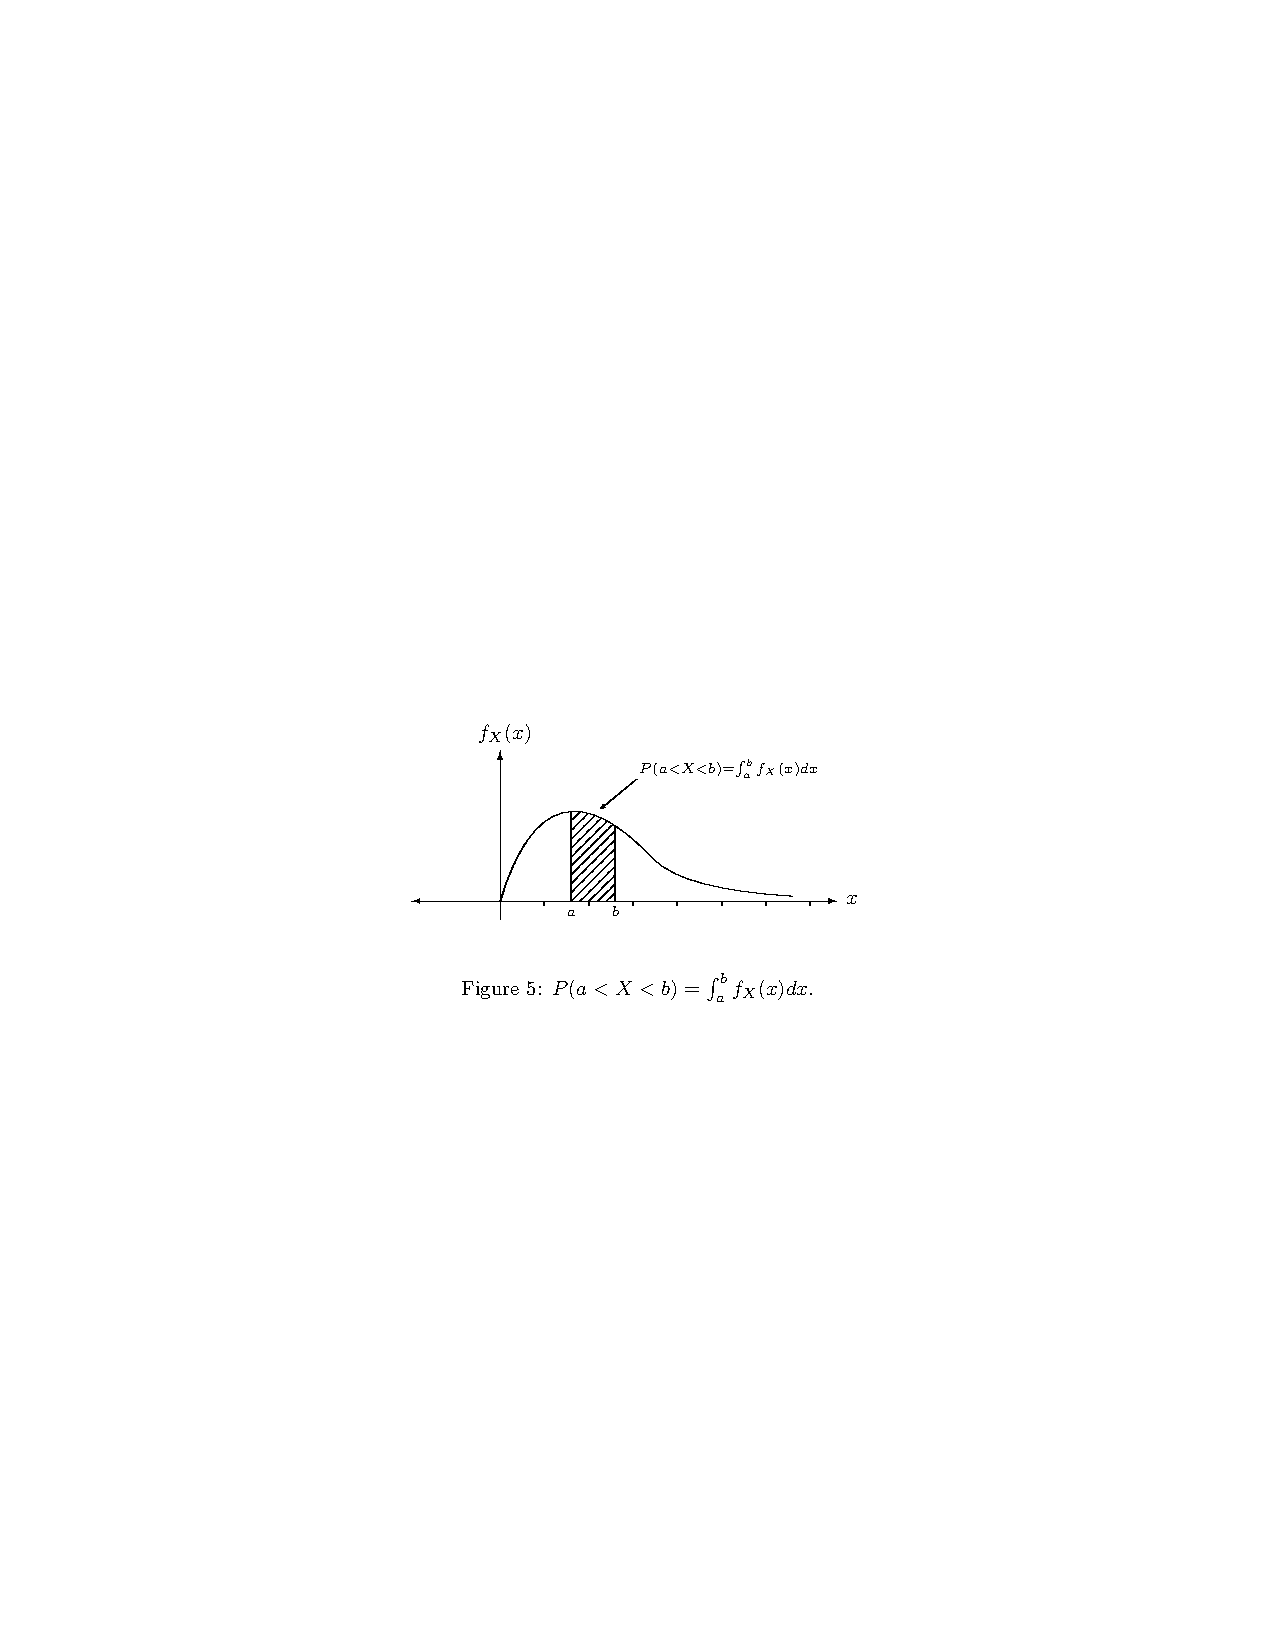
\includegraphics[width = 0.6\textwidth]{images/rec5_1}
\end{figure}
\end{frame}


\begin{frame}{The Normal Distribution}
\begin{itemize}
\setlength{\itemsep}{10pt}
\item A {\themecol normal} random variable is a continuous random variable.
\begin{figure}
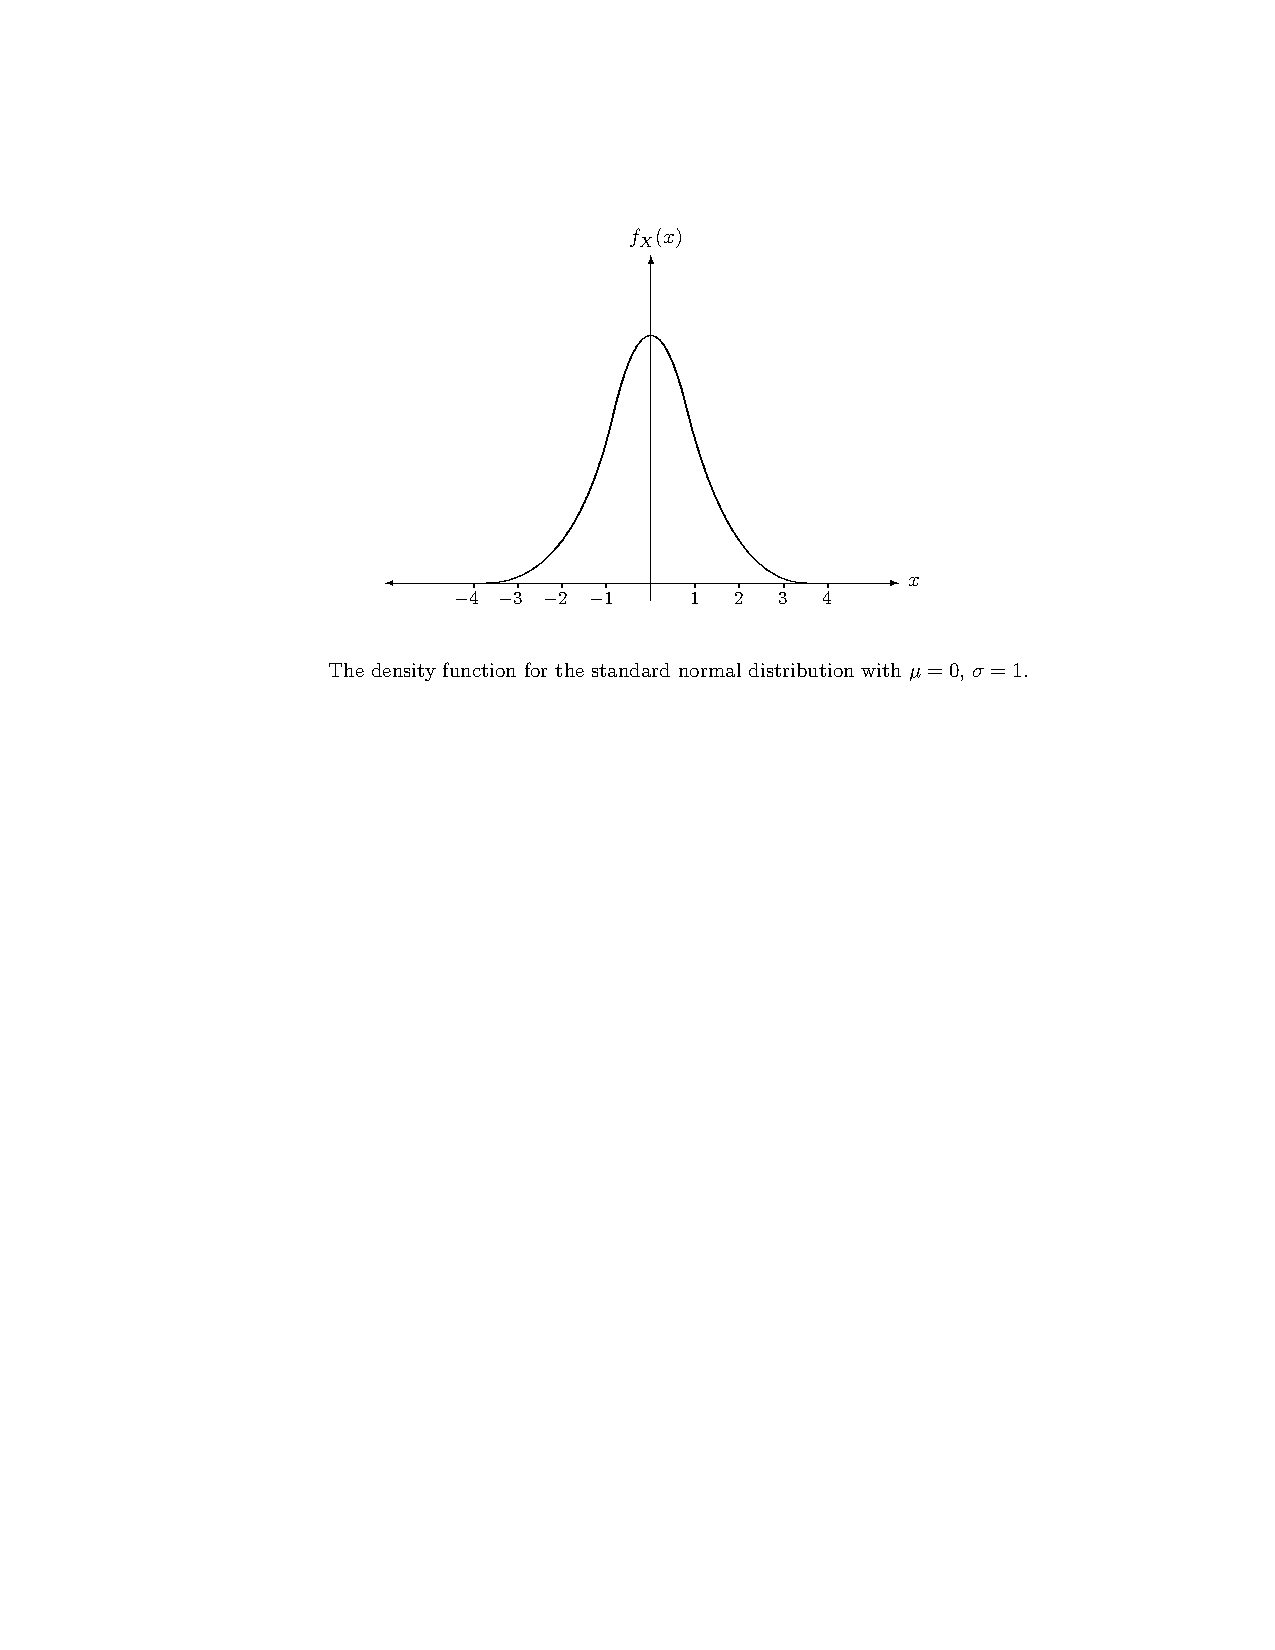
\includegraphics[width = 0.6\textwidth]{images/rec5_2}
\end{figure}
\item We call a normal random variable with $\mu = 0$ and $\sigma^2 = 1$ a {\themecol standard normal} random variable.
\item For standard normal random variables, we can use charts (or a computer) to find the area under the density function (i.e. the probabilities).
\end{itemize}
\end{frame}

\begin{frame}{Questions}
\begin{itemize}
\setlength{\itemsep}{15pt}
\item<1-> $P(Z < -1.75) $ 
\item<2->[] {\color{red}$P(Z < -1.75)= 0.0401$}
\item<3-> $P(Z > 0.85)$ 
\item<4->[]  {\color{red}$P(Z > 0.85)= 1- 0.8023 = 0.1977$}
\item<5->$ P(-1.43 < Z < 0.92) $
\item<6->[]  {\color{red}$P(-1.43 < Z < 0.92)  = 0.8212 - .0764 = .7448$}
\end{itemize}

\end{frame}

\begin{frame}{Standardization}
\begin{itemize}
\setlength{\itemsep}{20pt}
\item<1-> What if a normal random variable has a different mean and variance?
\item<2-> We need to \emph{standardize} it. 
\item<3-> Let $X \sim N(\mu, \sigma^2)$: that is, $X$ is a normal random variable with mean $\mu$, variance $\sigma^2$. Let
$$Z = \frac{X - \mu}{\sigma}$$
\item<4-> Then $Z$ is a \emph{standard} normal random variable.
\end{itemize}
\end{frame}

\begin{frame}{Example}
\begin{itemize}
\item<1-> $X$ is a normal random variable with $\mu = 5$ and $\sigma^2 = 9$. Find $P(X > 8)$.
\item<2->[] {\color{red}
\begin{align*}
P(X > 8) &= P\left( \frac{X-5}{3} > \frac{8 - 5}{3}\right)\\
&= P(Z > 1) \\
&= 0.1587
\end{align*}}
\end{itemize}
\end{frame}

\begin{frame}{Questions}
\begin{itemize}
\item<1-> $X \sim N(2, 16)$. Find $P(-1 < X < 6)$.
\item<2->[] \color{red}
\begin{align*}
P(-1 < X < 6 ) &= P\left(\frac{-1-2}{4} < \frac{X - 2}{4} < \frac{6 - 2}{4}\right) \\
&= P(-0.75 < Z < 1) \\
&= 0.8413 - 0.2266 \\
&= 0.6147
\end{align*} 
\end{itemize}
\end{frame}

\begin{frame}{Questions}
\begin{itemize}
\item<1-> $Y \sim N(7, 25)$. Find $P(8 < Y < 13)$.
\item<2->[] \color{red}
\begin{align*}
P(8 < Y < 13 )&= P\left(\frac{8 - 7}{5} < \frac{Y -7}{5}< \frac{13 - 7}{5}\right) \\
&= P(0.2 < Z < 1.2)\\
&= 0.8849 - 0.5793 \\
&= 0.3056
\end{align*}
\end{itemize}
\end{frame}

\begin{frame}{Two-Standard-Deviation Rule}
\begin{itemize}
\setlength{\itemsep}{15pt}
\item<1-> From the chart:
$$P(Z < -1.96) = 0.025, \quad P(Z > 1.96) = 0.025.$$
\item<2-> Then:
$$P(-1.96 < Z < 1.96) = 0.95.$$
\item<3-> Approximate $1.96 \approx 2$ and ``unstandardize":
$$P\left( -2 < \frac{X-\mu}{\sigma} < 2\right) = 0.95$$
\item<4->[$\Rightarrow$]  
$$P(\mu - 2\sigma < X < \mu + 2\sigma) = 0.95.$$
\item<5-> {\themecol The probability that a normal random variable is within 2 standard deviations of the mean is  $95\%$.} 
\end{itemize}
\end{frame}

\begin{frame}{Normal Distribution: Sums and Averages}
\begin{itemize}
\setlength{\itemsep}{15pt}
\item<1-> Let $X_1, \dots, X_n$ be independent and \emph{normally distributed}. Let 
$$T_n = X_1 + \cdots + X_n, \qquad \bar{X} = \frac{X_1 + \cdots X_n}{n}, \qquad D = X_2 - X_1.$$
\item<2-> Then $T_n$, $\bar{X}$ and $D$ are {\themecol also normal random variables}.
\item<3-> Let $X_1, \dots, X_n \stackrel{i.i.d}{\sim} N(\mu, \sigma^2)$. Then:
\begin{align*}
T_n &\sim N(n\mu, n\sigma^2)  \\[10pt]
 \overline{X} &\sim N\left(\mu, \frac{\sigma^2}{n}\right) \\[10pt]
D &\sim N(0, 2\sigma^2)
\end{align*}
\end{itemize}
\end{frame}

\begin{frame}{Example}
\begin{itemize}
\item Suppose we know the weight $X$ of an adult man chosen at random is normally distributed with mean 160 pounds and variance 64 pounds$^2$. \\[10pt]
\item[a)] Find $P(156 < X < 164)$.
\item<2->[] {\color{red} 
\vspace*{-0.25cm}
\begin{align*}
P(156 < X < 164) &= P\bigg(\frac{156-160}{8} < \frac{X - 160}{8} < \frac{164-160}{8}\bigg) \\
&= P(-0.5 < Z < 0.5) \\
&=  0.3830
\end{align*}}
\vspace*{-0.25cm}
\item<3->[b)] Find the probability that the average weight of 16 men chosen at random is between 156 and 164 pounds.
\vspace*{-0.25cm}
\item<4->[] \color{red}
\begin{align*}
\overline{X} &\sim N(160, 64/16 = 4) \\
P(156 < \overline{X} < 164) &= P(-2 < Z < 2)\\
&\approx 0.95
\end{align*}
\end{itemize}
\end{frame}

\begin{frame}{Example}
\begin{itemize}
\item Suppose we know the weight $X$ of an adult man chosen at random is normally distributed with mean 160 pounds and variance 64 pounds$^2$. \\[10pt]
\item[c)] Calculate the numbers $A$ and $B$ such that $P(A < X < B) \approx 0.95$.
\item<2->[] {\color{red} 
\vspace*{-0.25cm}
\begin{align*}
&0.95 \approx P\bigg(-2 < \frac{X-\mu}{\sigma} < 2\bigg) = P(-2\sigma + \mu < X < 2\sigma + \mu) \\
&A = -2(8) + 160 = 144,  \quad B = 2(8) + 160 = 176
\end{align*}}
\vspace*{-0.25cm}
\item<3->[d)] Calculate the numbers $C$ and $D$ such that the average of 256 randomly chosen adults is between $C$ and $D$ with probability approximately 0.95.
\item<4->[] {\color{red}
\vspace*{-0.5cm}
\begin{align*}
&\overline{X}_{256} \sim N(160, 64/256 = 1/4) \\
&C = -2\sigma + \mu = -2(1/2) + 160 = 159 \\
&D = 2\sigma + \mu = 2(1/2) + 160 = 161
\end{align*}}
\vspace*{-0.25cm}
\end{itemize}
\end{frame}

\begin{frame}{Central Limit Theorem}
\begin{itemize}
\setlength{\itemsep}{15pt}
\item[] {\themecol The Central Limit Theorem:}
\item Suppose $X_1, X_2, \dots, X_n$ are \emph{iid} with mean $\mu$ and variance $\sigma^2$. 
\item Then, for large $n$
\begin{align*}
\themecol T_n \sim N(n\mu, n\sigma^2)\quad \text{and} \quad \bar{X} \sim N\left(\mu, \frac{\sigma^2}{n}\right)
\end{align*}
{\centering \emph{no matter the distribution of the individual} $X_i$}
\item Allows approximation of all distributions using the normal distribution if you know the mean and variance.
\item<2->[Note:] \small if $X_1, \dots, X_n$ are normally distributed, then this applies for \emph{all} $n$, not just large $n$.
\end{itemize}
\end{frame}

\begin{frame}{Central Limit Theorem: Example}
\begin{itemize}
\setlength{\itemsep}{15pt}
\item<1-> Let $X_1, X_2,\dots, X_n \stackrel{iid}{\sim} Binomial(1, \theta)$.
\item<2-> For each $X_i$, $Mean(X_i) = \theta$ and $Var(X_i) = \theta(1-\theta).$
\item<3-> The sum is: $T_n = X_1 + X_2 + \cdots + X_n$.
\item<4-> The proportion is:
 $$P = \frac{X_1 + \cdots + X_n}{n}.$$
\item<6-> For large $n$, 
\begin{align*}
T_n &\sim N\left(n\theta, n\theta[1-\theta]\right) \\[1.5 em]
P &\sim N\left( \theta, \frac{\theta(1-\theta)}{n}\right)
\end{align*}
\end{itemize}
\end{frame}

\begin{frame}{Central Limit Theorem: Problem}
\begin{itemize}
\item<1-> Suppose you are rolling a fair die 1000 times. Calculate the numbers $A$ and $B$ such that the average of the 1000 rolls is between $A$ and $B$ with probability approximately 0.95. You may assume the mean of one roll is 3.5 and the variance is 35/12.
\item<2->[] {\color{red}
\vspace*{-0.5cm}
\begin{align*}
&Mean(X_i) = 3.5, \quad Var(X_i) = 35/12 \\
&\overline{X} \sim N\bigg(\mu, \frac{\sigma^2}{n}\bigg) = N\bigg(3.5, \frac{35}{12000} \bigg) \quad \text{by CLT}\\
&A = -2\sigma + \mu = -2\sqrt{35/12000} + 3.5 \approx 3.392 \\
&B = 2\sigma + \mu = 2\sqrt{35/12000} + 3.5 \approx 3.608
\end{align*}}
\vspace*{-0.25cm}
\end{itemize}
\end{frame}





\end{document}


